\documentclass[a4paper,11pt]{article}

\usepackage[utf8x]{inputenc}
\SetUnicodeOption{mathletters}
\SetUnicodeOption{autogenerated}

\usepackage[italian]{babel}
\usepackage{booktabs}
\usepackage{mathpazo}
\usepackage{graphicx}
\usepackage[left=2cm, right=2cm, bottom=3cm]{geometry}
\frenchspacing

\begin{document}
\noindent {\Large Selezioni Territoriali 2012}
\vspace{0.5cm}

\noindent {\Huge Il tesoro del Pirata Barbablù (\texttt{barbablu})}


\vspace{0.5cm}
\noindent {\Large Difficoltà D = 2.}

\section*{Descrizione del problema}
  
John Steam della compagnia "Oriental Steam Navigation" decide di
organizzare una spedizione di recupero del tesoro del Pirata Barbablù,
custodito nel relitto del galeone del pirata, affondato al largo di
Gobal, che si trova adagiato su un fianco a 30 metri di profondità.
L'unico punto di accesso al relitto è uno squarcio sulla fiancata, in
corrispondenza della cabina numero 1. Nel galeone sono presenti cabine e
corridoi che le collegano. Tutti i corridoi sono totalmente sommersi
dall'acqua a causa della rottura degli oblo mentre in alcune delle
cabine sono rimaste delle sacche d'aria. A causa degli spazi angusti non
è possibile, per i sommozzatori, esplorare la nave con le bombole
d'aria; sono quindi costretti a nuotare in apnea, sfruttando le sacche
d'aria presenti nel tragitto per respirare. 
        
Prima di procedere con le operazioni di recupero ti viene commissionata
la realizzazione di un programma in grado di individuare il percorso più
breve all'interno del galeone che permetta ai sommozzatori di
raggiungere la cabina con il tesoro a partire dall'apertura.  In alcune
cabine sono presenti sacche d'aria che possono essere usate per
respirare. Un sommozzatore riesce a nuotare senza aria per 20 metri al
massimo prima di dover riprendere fiato.  In Figura 1 sono mostrati due
possibili scenari. La cabina di ingresso è come detto la numero 1,
mentre la cabina del tesoro (rappresentato da una T) è la numero 2 per
l'esempio di sinistra, e la numero 4 per l'esempio di destra. Le cabine
con la sacca d'aria sono quadrate, mentre quelle senza sacca sono tonde.
A fianco di ogni corridoio è segnata la sua lunghezza in metri.
L'esempio di sinistra ammette una sola soluzione, di lunghezza 29 metri,
mentre quello di destra non ha soluzioni.
        
\begin{figure}[h!] \centering \caption{} 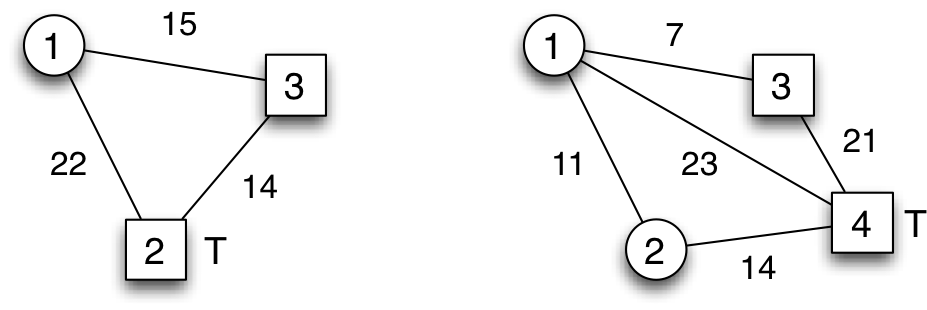
\includegraphics{mappa.png}
\end{figure}

Le cabine della nave sono numerate da 1 ad $N$ e sono collegate tra loro
da $M$ corridoi.  L'apertura  è la numero 1 mentre il tesoro si trova
nella cabina numero $C$ (con 1 ≤ $C$ ≤ $N$).  Di ogni cabina si conosce
l'eventuale presenza di aria e di ogni corridoio la lunghezza in metri.
        
Il tuo compito è quello di trovare la lunghezza in metri del percorso
più breve che permette ad un sommozzatore di partire dalla cabina con
l'apertura e di raggiungere il tesoro, in apnea, sfruttando le eventuali
sacche d'aria trovate nel percorso. La cabina del tesoro ha sempre una
sacca d'aria, che consente al sommozzatore di recuperare il tesoro.
        

\section*{Dati di input}
  
Il file \texttt{input.txt} è composto da $M$+2 righe. La prima riga
contiene quattro interi positivi separati da uno spazio, che
rappresentano il numero $N$ delle cabine, il numero $M$ dei corridoi, il
numero $C$ che rappresenta la cabina del tesoro e il numero $K$ che
rappresenta quante cabine hanno sacche d'aria al loro interno.  La
seconda riga contiene $K$ numeri separati da uno spazio che
rappresentano i numeri (distinti) delle cabine che contengono aria.
Ciascuna delle rimanenti $M$ righe contiene tre interi $I$,$J$, $L$
separati da uno spazio che indicano la presenza di un corridoio che
collega le cabine $I$ e $J$ di lunghezza $L$ (in metri).

\section*{Dati di output}
  
Il file \texttt{output.txt} è composto da una sola riga contenente la
lunghezza in metri del percorso più breve che permetta, a partire
dall'apertura, di raggiungere la cabina del tesoro in apnea.  Riportare
-1 se non esiste nessun percorso che soddisfa i vincoli.

        
\section*{Assunzioni}
\begin{itemize}
  \item $2 ≤ N ≤ 30$
  \item $2 ≤ M ≤ 100$
  \item $1 ≤ C ≤ N$
  \item $0 ≤ K ≤ N$
\end{itemize}

\section*{Esempi di input/output}
    \noindent
    \begin{tabular}{p{11cm}|p{5cm}}
    \toprule
    \textbf{File \texttt{input.txt}}
    & \textbf{File \texttt{output.txt}}
    \\
    \midrule
    \scriptsize
    \begin{verbatim}
            3 3 2 2
            2 3
            1 2 22
            1 3 15
            2 3 14
            \end{verbatim}
    &
    \scriptsize
    \begin{verbatim}
            29
            \end{verbatim}
    \\
    \bottomrule
    \end{tabular}
  
    \noindent
    \begin{tabular}{p{11cm}|p{5cm}}
    \toprule
    \textbf{File \texttt{input.txt}}
    & \textbf{File \texttt{output.txt}}
    \\
    \midrule
    \scriptsize
    \begin{verbatim}
            4 5 4 2
            3 4
            1 2 11
            1 3 7
            1 4 23
            2 4 14
            3 4 21
            \end{verbatim}
    &
    \scriptsize
    \begin{verbatim}
            -1
            \end{verbatim}
    \\
    \bottomrule
    \end{tabular}

\end{document}
